%! Author = Omar Iskandarani
%! Title = Einstein and the Æther: A Philosophical Foundation for the Vortex Æther Model (VAM)
%! Date = May 23, 2025
%! Affiliation = Independent Researcher, Groningen, The Netherlands
%! License = CC-BY 4.0
%! ORCID = 0009-0006-1686-3961
%! DOI = 10.5281/zenodo.15566101

\documentclass[a4paper,12pt]{article}

% Page Geometry
\usepackage[a4paper, margin=2cm]{geometry}
\usepackage[utf8]{inputenc}
\usepackage[T1]{fontenc}
% Language, Encoding, Fonts

\usepackage{lmodern}
\usepackage[english]{babel}

% Colors, Graphics, Diagrams
\usepackage{graphicx}
\usepackage{tikz}
\usetikzlibrary{arrows.meta, positioning}
\usepackage{pgfplots}
\pgfplotsset{compat=1.18}
\usepackage{xcolor}

\usepackage{amssymb}

\usepackage{physics}

\usepackage{em}

\usepackage[font=footnotesize]{caption}
% Math and Physics
\usepackage{amsmath, amssymb, physics}
\usepackage{siunitx}

% Tables and Figures
\usepackage{float}
\usepackage{booktabs}
\usepackage{array, tabularx, makecell, multirow}
\renewcommand{\arraystretch}{1.5}
\renewcommand{\floatpagefraction}{.8}

\usepackage{subcaption}

% Code and Listings
\usepackage{listings}
\lstset{basicstyle=\ttfamily\footnotesize, breaklines=true}

% TOC Customization
\usepackage{tocloft}
\setcounter{tocdepth}{4}
\renewcommand{\cftsecfont}{\bfseries}
\renewcommand{\cftsubsecfont}{\itshape}
\renewcommand{\cftsecleader}{\cftdotfill{5}}
\renewcommand{\contentsname}{\centering \Huge\textbf{Contents}}

% Links and Metadata
\usepackage{hyperref}
\hypersetup{
    colorlinks=true,
    linkcolor=blue,
    citecolor=blue,
    urlcolor=blue,
    pdftitle={The Vortex Æther Model},
    pdfauthor={Omar Iskandarani},
    pdfkeywords={vorticity, gravity, æther, fluid dynamics, time dilation, VAM}
}
\usepackage{bookmark} % PDF bookmarks


\usepackage[most]{tcolorbox}
\tcbuselibrary{listings, breakable, skins}

\newtcolorbox{vamprinciple}[1][]{
    enhanced,
    breakable,
    colback=blue!5!white,
    colframe=blue!60!black,
    fonttitle=\bfseries,
    title=Hybrid Gravitational Coupling in the Vortex Æther Model,
    coltitle=black,
    #1
}


% Line and Hyphenation
\usepackage[none]{hyphenat}
\usepackage{amsfonts}
\usepackage{sectsty}
\sectionfont{\Large\bfseries\sffamily}
\subsectionfont{\large\bfseries\sffamily}
\usepackage{newtxtext,newtxmath}
\usepackage[scaled=0.95]{inconsolata} % for a clean monospace font
\usepackage{mathrsfs}
% Bibliography

\begin{document}


    \begin{table}[h]
        \centering
        \begin{tabular}{|l|c|l|p{7cm}|}
            \hline
            \textbf{Name} & \textbf{Symbol} & \textbf{Type} & \textbf{Description and Role} \\
            \hline
            Chronos-time & $\tau$ & Relative / Measurable & Sequential time; proper time experienced by localized systems in motion through the æther. Core for modeling time dilation. \\
            \hline
            Aithēr-time & $\mathcal{N}$ & Absolute / Universal & The invariant universal present; a metaphysical and ontological background for all temporal flow. \\
            \hline
            Swirl Clock & $\circlearrowleft$ or $S(t)$ & Local / Cyclical & Internal clock-like rhythm of a vortex knot. Tracks phase, rotation, or identity shift through time. \\
            \hline
            Kairos Moment & $\mathbb{K}$ & Threshold / Emergent & The qualitative, transformational moment when a system undergoes critical phase alignment or collapse. \\
            \hline
            Æther Frame & $\Xi_0$ & Reference Frame & Hypothetical inertial frame where the æther medium is at rest. Used for symmetry-breaking and baseline flow analysis. \\
            \hline
            Vortex Proper Time & $T_v$ & Derived / Topological & Time internal to the closed knot or vortex loop. Emerges from geodesic paths and twist topology. \\
            \hline
            Now-Point & $\nu_0$ & Local Event / Temporal Slice & Precise location in spacetime where a point in the æther intersects the universal present. Useful in field causality. \\
            \hline
        \end{tabular}
        \caption{Temporal constructs used in the Vortex Æther Model. These notations distinguish between measurable time, absolute background time, internal vortex phase, and field-causality moments.}
        \label{tab:VAM_time}
    \end{table}

    \begin{align}
        \text{(1) Vortex Proper Time Evolution:}\\
        \quad & \dv{\tau}{\mathcal{N}} = \gamma^{-1}(\vec{v}) \\
        \text{(2) Swirl Clock Gradient:}\\ \quad & \nabla S(t) = \frac{\partial \vec{S}}{\partial \mathcal{N}} + \omega(\tau) \hat{n} \\
        \text{(3) Field Tensor Modulation (Æther-relative):} \\\quad & F^{\mu\nu}(\Xi_0) = \partial^\mu A^\nu - \partial^\nu A^\mu + \phi(\circlearrowleft) \delta^{\mu\nu} \\
        \text{(4) Ætheric Causality Surface:}\\ \quad & \Sigma_{\nu_0} = \{ x^\mu \ | \ \tau(x) = \mathcal{N} \} \\
        \text{(5) VAM Energy Conservation in Æther Frame:}\\ \quad & \dv{E}{\mathcal{N}} + \nabla \cdot \vec{J} = \mathbb{K}(\vec{x}, \tau)
    \end{align}


\section*{🔀 Classical Greek Candidates}
\subsection*{✅ χρόνος (Chronos) — \textit{Linear time}}
\begin{itemize}
\item Sequential, measurable
\item Already used in physics-adjacent language
\item Good for Swirl Clocks
\end{itemize}

\subsection*{✅ καιρός (Kairos) — \textit{Qualitative, sacred, the right time}}
\begin{itemize}
\item Evokes \textit{timelessness} or \textit{significance}
\item Works for moments of change, turning points, or \textit{the now}
\item A good poetic stand-in for absolute time, but maybe too mystical
\end{itemize}

\subsection*{🚫 ὥρα (Hora) — Kind of basic}
\begin{itemize}
\item Literally “hour”
\item Probably \textit{too} mundane unless you’re naming a clock app
\end{itemize}


\section*{🧠 Wild but Useful Alternatives}
\subsection*{✅ Αἰθήρ (Aithḗr) — literally “Æther”}
\begin{itemize}
\item Why not just \textit{own} it? Make Aithēr-time the name of the universal backdrop
\item Then Chronos-time becomes the local, measurable perturbation
\item Let the reader \textit{feel} that difference:
\begin{itemize}
\item "In Aithēr-time, all events coexist."
\item "In Chronos-time, your wristwatch disagrees with my satellite."
\end{itemize}\end{itemize}

\subsection*{✅ Νῦν (Nun) — “Now”, in philosophical Greek}
\begin{itemize}
\item Used heavily in Aristotle for the "eternal now"
\item Could be a poetic alias for the presence-point in your model
\end{itemize}




Get real spicy and use:


\begin{itemize}
\item ⊚ for the universal present
\item Δτ for local proper time changes
\item 𝕂 for Kairos-time when something irreversible happens
\end{itemize}




\begin{table}
    \centering
    \begin{tabular}{llll}
        \toprule
        \textbf{Concept} & \textbf{Word} & \textbf{Symbol Suggestion} & \textbf{Notes} \\
        \midrule
        Relative Time & Chronos & τ (tau) & Already used for proper time in relativity. Feels right. \\
        Absolute Time & Aithēr-Time or Nun & 𝒩 or 𝔄 (calligraphic N or A) & Stands for “Now” or “Æther.” Visually distinct. \\
        Swirl Clock & – & ⟳ or 𝛀 (Omega) & Circular, cycle-based. Maybe use for specific time dilation rings. \\
        Absolute Frame & – & Ξ (Xi) or Ω₀ & Could designate the undisturbed æther frame. \\
        \bottomrule
    \end{tabular}
    \caption{}
    \label{tab:}
\end{table}

    \begin{figure}[h!]
        \centering
        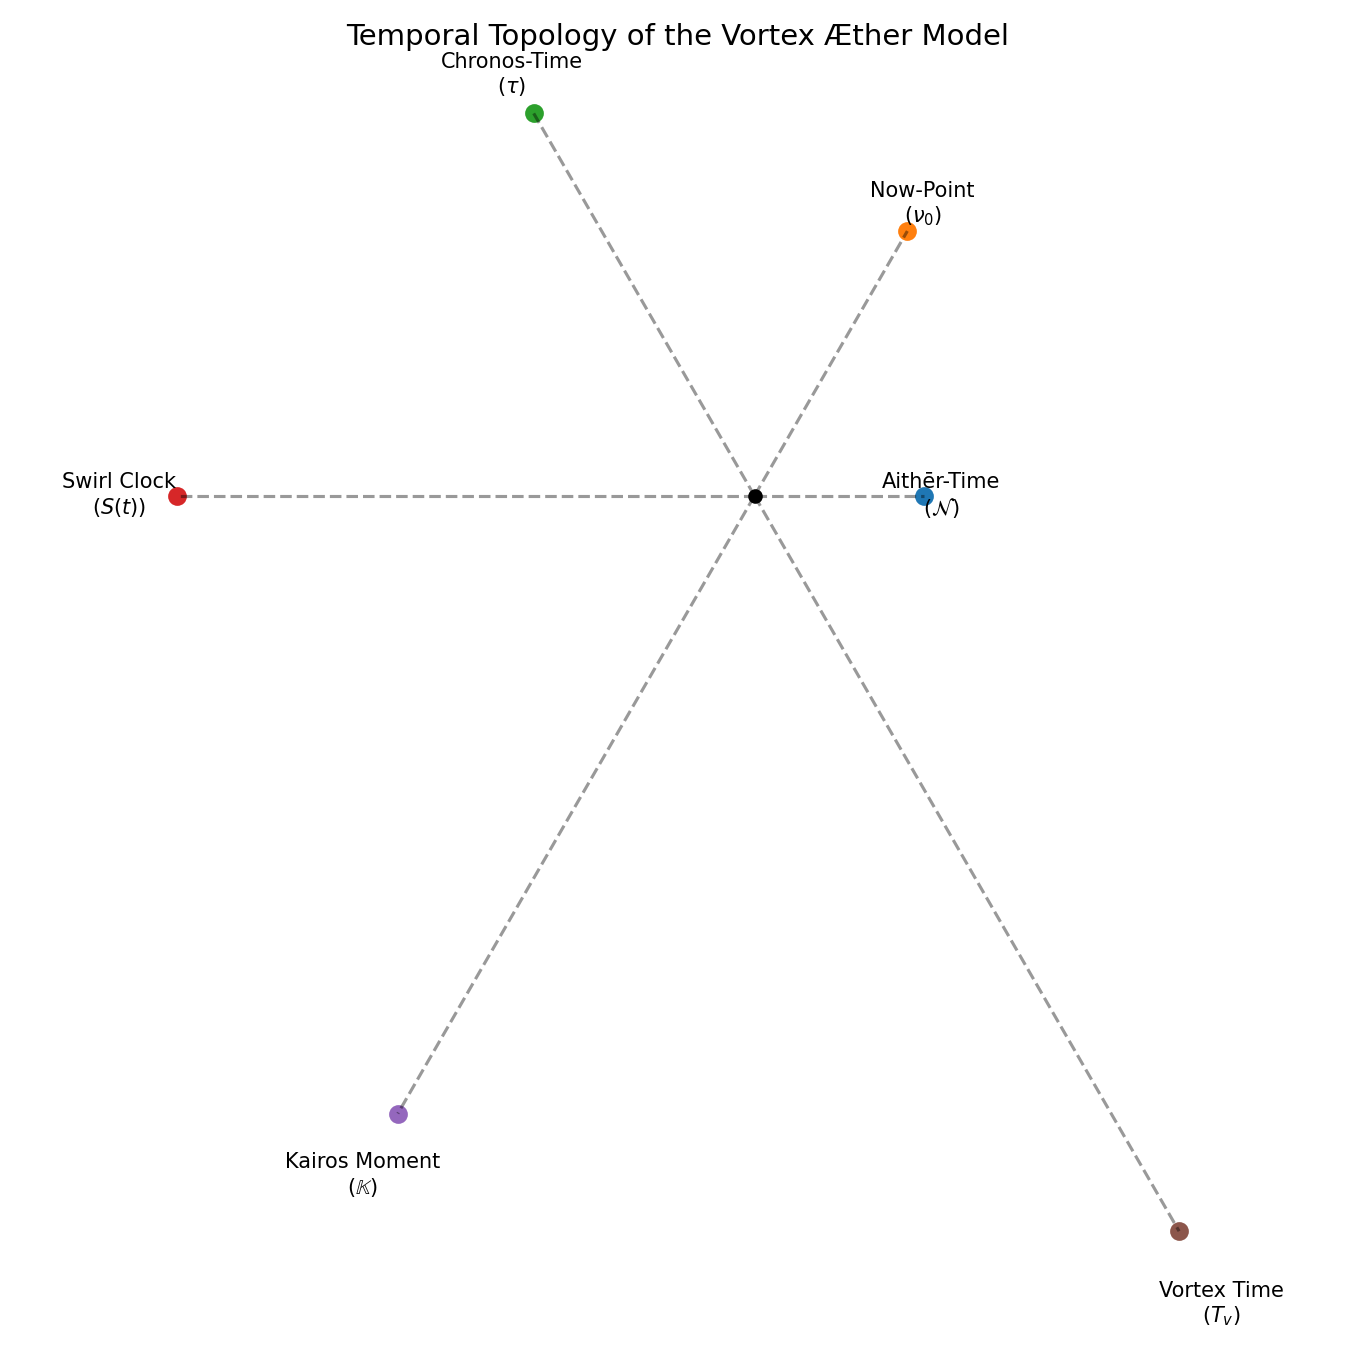
\includegraphics[width=0.65\textwidth]{TimeConstruct} % insert your generated swirl diagram here
        \caption{Temporal Topology in the Vortex Æther Model (VAM). All constructs of time emerge radially from a central ætheric origin. Each node represents a different mode of temporal existence in the VAM framework.}
        \label{fig:VAM-time-swirl}
    \end{figure}

    \subsection*{Interpretation of the Temporal Swirl}

    The Vortex Æther Model introduces a layered ontology of time, expressed visually as a topological swirl. At the origin lies the metaphysical æther, an inertial and undisturbed medium. From this foundation, distinct temporal modes unfold:

    \begin{itemize}
        \item \textbf{Aithēr-Time (\( \mathcal{N} \))}: The universal, absolute timeline. Serves as a background structure for causality and all field dynamics. Not experienced directly but used as a reference.
        \item \textbf{Now-Point (\( \nu_0 \))}: A local intersection in spacetime where an event coincides with the universal present. Defines causal update surfaces.
        \item \textbf{Chronos-Time (\( \tau \))}: Measurable time within the ætheric flow. Corresponds to proper time and exhibits relativistic effects such as dilation.
        \item \textbf{Swirl Clock (\( S(t) \))}: Internal phase tracker of a vortex. Encodes identity, rotation, and the cumulative effect of angular motion.
        \item \textbf{Kairos Moment (\( \mathbb{K} \))}: Topological or energetic bifurcation points. Used to mark critical transitions like reconnection or collapse.
        \item \textbf{Vortex Proper Time (\( T_v \))}: The geodesic loop-time inside a vortex. It is a derived, topological measure based on internal circulation or twist count.
    \end{itemize}

    Each form of time in the VAM supports a different domain of analysis: from global conservation and symmetry breaking to local measurement and knot identity. By using this temporal taxonomy, the model bridges metaphysical continuity with emergent topological structure. This multi-layered treatment is essential for describing phase shifts, causality, and stability in vortex-bound field dynamics.




    \begin{sidewaystable}
        \centering
        \scriptsize
        \begin{tabular}{|l|l|l|l|l|l|l|}
            \hline
            \textbf{} & \textbf{Aithēr-Time} (\(\mathcal{N}\)) & \textbf{Now-Point} (\(\nu_0\)) & \textbf{Chronos-Time} (\(\tau\)) & \textbf{Swirl Clock} (\(S(t)\)) & \textbf{Kairos Moment} (\(\mathbb{K}\)) & \textbf{Vortex Time} (\(T_\text{v}\)) \\
            \hline
            \textbf{Aithēr-Time (𝒩)} & Universal backdrop; absolute & Defines when Now-point is sampled & Chronos is a projection from 𝒩 & Phase progresses within 𝒩 flow & Kairos occurs within 𝒩 but is nonlinear & T\textsubscript{v} is measured relative to 𝒩 \\
            \hline
            \textbf{Now-Point (ν₀)} & Sampled slice of 𝒩 & Event intersection; singular & Local instance where τ = 𝒩 & Marks phase readout point & Moment of phase collapse & Entry/exit point on vortex loop \\
            \hline
            \textbf{Chronos-Time (τ)} & Relative clock derived from 𝒩 & Progresses across ν₀ slices & Classical relativistic time & Phase unfolds at rate tied to τ & Events emerge when τ hits critical & External view of internal vortex \\
            \hline
            \textbf{Swirl Clock (S(t))} & Phase tracker on 𝒩 base & Sampled at ν₀ per loop & Depends on τ to accumulate phase & Cyclic identity; angular continuity & Phase jump marks kairotic moment & Loops with twist and rotation \\
            \hline
            \textbf{Kairos Moment (𝕂)} & Nonlinear fold in 𝒩 & Qualitative event at ν₀ & Threshold within τ evolution & Phase alignment triggers 𝕂 & Collapse/transition point & Time bifurcation on vortex \\
            \hline
            \textbf{Vortex Time (T\textsubscript{v})} & Looped time span via 𝒩 & Now-point traced along knot & τ projected over closed path & Builds S(t) over knot period & Marks full-cycle threshold & Geodesic knot duration \\
            \hline
        \end{tabular}
        \caption{Comparison matrix of temporal constructs in the Vortex Æther Model (VAM), showing how each concept interrelates with the others.}
    \end{sidewaystable}
    \section*{Temporal Constructs in the Vortex Æther Model (VAM)}

    \subsection*{🌌 Aithēr-Time $\mathcal{N}$ — Absolute Background Time}
    \textbf{Concept:} The universal, nonlocal flow of time; the foundation from which all other temporal phenomena are derived.

    \textbf{Mathematical Form:}
    \[
        \mathcal{N} \in \mathbb{R}, \quad d\mathcal{N} = \text{invariant}
    \]

    \textbf{Physical Role:} Provides the absolute time frame used to define causality and field evolution in the æther medium.

    \textbf{Applications:} Symmetry foundations, æther dynamics, background for field interactions.

    \subsection*{🕳️ Now-Point $\nu_0$ — Local Present Intersection}
    \textbf{Concept:} The intersection of a system with the absolute time—defining its local "now."

    \textbf{Mathematical Form:}
    \[
        \nu_0(x) : \tau(x) = \mathcal{N}
    \]

    \textbf{Physical Role:} Anchors relativistic causality. Each observer's "present" exists as a now-point in the universal flow.

    \textbf{Applications:} Event tracking, synchronization, slice definitions in relativistic spacetime.

    \subsection*{🔁 Swirl Clock $S(t)$ — Phase Evolution, Continuous Identity}
    \textbf{Concept:} The cyclic time evolution of a vortex; a phase tracker or heartbeat of the vortex.

    \textbf{Mathematical Form:}
    \[
        S(t) = \theta(t) \mod 2\pi
    \]

    \textbf{Physical Role:} Represents the local angular phase of the vortex; tracks internal identity through cyclic motion.

    \textbf{Applications:} Rotational symmetry, Berry phase analogs, spin coherence.

    \subsection*{🔄 Vortex Time $T_v$ — Topological Duration, Internal Clock}
    \textbf{Concept:} The intrinsic looped time experienced by a vortex through one full geodesic cycle.

    \textbf{Mathematical Form:}
    \[
        T_v = \oint \frac{ds}{v_{\text{phase}}}
    \]

    \textbf{Physical Role:} Measures internal duration of a knot loop; basis for vortex identity and mass stability.

    \textbf{Applications:} Quantized circulation, knot dynamics, resonance time, mass derivation.

    \subsection*{⏳ Chronos-Time $\tau$ — Measurable, External Flow}
    \textbf{Concept:} Classical proper time experienced by moving bodies, projected from the universal frame.

    \textbf{Mathematical Form:}
    \[
        d\tau = \frac{1}{\gamma(\vec{v})} d\mathcal{N}
    \]

    \textbf{Physical Role:} Governs relativistic time dilation and clock rates in the moving æther frame.

    \textbf{Applications:} Lorentz transformations, motion analysis, æther-relative physics.

    \subsection*{💥 Kairos Moment $\mathbb{K}$ — Transformational Threshold}
    \textbf{Concept:} A phase-critical moment in which irreversible change or collapse occurs.

    \textbf{Mathematical Form:}
    \[
        \mathbb{K}(\vec{x}, \tau) = \delta(\tau - \tau_c)
    \]

    \textbf{Physical Role:} A singular moment of transition—birth, collapse, phase shift, or knot reconnection.

    \textbf{Applications:} Discrete jumps in vortex state, mass bifurcation, ætheric events.



\end{document}